\documentclass[a4paper,11pt,parskip]{scrartcl}
\usepackage[utf8]{inputenc}
\usepackage[ngerman]{babel}
\usepackage[T1]{fontenc}
\usepackage{lmodern}
\usepackage{amsmath}
\usepackage{amsfonts}
\usepackage{amssymb}
\usepackage{amsthm}
\usepackage{siunitx}
\usepackage{epsfig}
\usepackage{url}
\usepackage{tikz}
\usepackage[lined,algoruled,linesnumbered]{algorithm2e}
%% \usepackage{algpseudocode}
%% \usepackage{algorithm}
\usepackage{graphicx}
\usepackage{placeins}

% an seitenbreite angepasste tabellen
\usepackage{booktabs}
\usepackage{tabularx} % page-width
\usepackage{adjustbox}

% coole inline-todos :)
\usepackage[colorinlistoftodos,prependcaption]{todonotes}

% Zeilenabstand
\usepackage[onehalfspacing]{setspace}

% PDF Bookmarks
\usepackage[backref=true,pagebackref=true,colorlinks=false,bookmarks=true,bookmarksopen=false,bookmarksnumbered=false,pdfpagemode=None]{hyperref}

% Seitenränder
\usepackage{geometry}             % Satzspiegel festlegen
\geometry{left=3cm, right=2.5cm, top=3cm, bottom=2cm, foot=1cm}

% Typographie: Besseres Absatz-Handling, größere Toleranzen beim Blocksatz
\tolerance 1414
\hbadness 1414
\emergencystretch 1.5em
\hfuzz 0.3pt
\widowpenalty=10000               % Hurenkinder vermeiden
\displaywidowpenalty=10000        % Hurenkinder vermeiden
\clubpenalty=10000                % Schusterjungen vermeiden
\vfuzz \hfuzz
\raggedbottom

\renewcommand{\arraystretch}{1.5}

\usetikzlibrary{shapes.geometric, positioning, calc, shapes, fit, backgrounds}

\title{Projektausarbeitung \\\vspace{.5cm} \large gt Scaffolder: Eine Scaffolding-Software}

\author{Dorle Osterode, Lukas Götz \& Stefan Dang}
\date{}

\begin{document}
\maketitle{}
\thispagestyle{empty}
\begin{abstract}
  \todo{wollen wir ein abstract haben?}
\end{abstract}

\newpage{}
\thispagestyle{empty}
\tableofcontents{}
\newpage{}
\setcounter{page}{1}
\section{Einleitung}

Das Ziel einer DNA-Sequenzierung ist die Bestimmung der Basen-Abfolge
der vorliegenden DNA. Moderne Sequenzierungstechniken, auch
\textit{Next-Generation Sequencing} genannt, können auch Read-Paare
produzieren. Dabei werden jeweils beide Enden eines DNA-Fragments
sequenziert. Abhängig vom verwendeten Sequenzierungsprotokoll
überbrücken gepaarte Reads Lücken (Inserts) variabler Größe.

Zur Rekonstruktion der Zielsequenz aus den Reads unabhängig von einer
Referenzsequenz kann eine \textit{de novo} Assemblierung durchgeführt
werden. Typischerweise wird hierbei in zwei Schritten vorgegangen:
Zunächst werden die einzelnen Reads zu durchgängigen Sequenzen
(Contigs) assembliert. Dabei kann das Zielgenom oftmals nicht
vollständig rekonstruiert werden. Aufgrund teilweise unzureichender
Abdeckung durch die Sequenzierung sowie repetitiver Teilsequenzen
entstehen Lücken (Gaps), welche zu unabhängigen Contigs führen. Die
relative Anordnung und Orientierung der Contigs zueinander kann nicht
bestimmt werden.

Durch \textit{Paired-End}- oder \textit{Mate-Pair}-Sequenzierung
gewonnene Reads können auf unterschiedlichen Contigs liegen und so
eine Beziehung zwischen diesen herstellen. Im zweiten Schritt einer
\textit{de novo} Assemblierung können diese Distanzinformationen dazu
verwendet werden, um die Contigs in Scaffolds anzuordnen. Dies erhöht
die Durchgängigkeit der assemblierten Sequenz. Scaffolds bestehen
dabei aus einer Reihe von geordneten Contigs, deren Distanz und
relative Orientierung festgelegt werden.

Das Scaffolding Problem kann als graphentheoretisches Problem
formuliert werden. Dabei repräsentieren die Knoten des Graphen die
einzelnen Contigs. Zwischen zwei Knoten existiert eine Kante, falls
ein Read-Paar die beiden repräsentierten Contigs verbindet. Kanten
enthalten hierbei Informationen über die Distanz der verbundenen Contigs
und die Orientierung der Read-Paare zueinander. Die Ermittlung eines
Scaffolds bzw.\ eines optimalen Pfades (Pfad mit maximalem Kantengewicht)
jeder Zusammenhangskomponente des Scaffolding Graphen, ist
NP-vollständig~\cite{Huson:2002kf}. Daher verwenden aktuelle
Strategien eine Heuristik, um einen guten Pfad zu
bestimmen.

Diese Ausarbeitung beschäftigt sich mit der Implementation eines
Scaffolding-Programms im Rahmen des Genominformatik-Projektes. Die
Implementation und komplette Dokumentation ist unter
\url{https://github.com/dorleosterode/gt-scaffold} zu finden. Der Fokus der
Ausarbeitung liegt auf der zugrunde liegenden Methodik. Für
Implementationsdetails steht der Source Code-Code zur Verfügung.

\section{Ziel des Projektes und Arbeitsvorgehen}
\subsection{Ziel des Projektes}
Die Implementierung und Evaluierung einer Scaffolding-Software stellte
das allgemeine Projektziel dar. Dabei sollten die in der
GenomeTools-Bibliothek~\cite{Gremme:2013} vorhandenen Konzepte und
Infrastruktur verwendet und eine Kompatibilität mit den Ausgaben des
Assemblers Readjoiner~\cite{Gonnella:2012gn} gewährleistet werden. Der
Scaffolder aus dem SGA-Softwarepaket~\cite{Simpson:2012ef} sollte als
Vorlage dienen, da diese Software im Rahmen einer Untersuchung
verschiedener Scaffolding-Programme Ergebnisse mit besonders hoher
Qualität lieferte~\cite{Hunt:2014dh}. Andererseits enthält
SGA-Scaffold zahlreiche Abhängigkeiten zu nicht-Standardsoftware, die
durch die Reimplementierung minimiert werden sollten. Dazu gehört zum
Beispiel, dass zur Ermittelung der Distanzinformationen eine Zuordnung
der Reads zu den Contigs auf Basis des String-Graphen erfolgt anstelle
eines Read-Mappings durch BWA~\cite{Li:2009}. Des Weiteren existiert
keine hinreichende Dokumentation der Methodik von SGA-Scaffold, so
dass dessen Aufklärung einen zentralen Teil des Projektes umfasste.

\subsection{Arbeitsvorgehen}
Die erste Aufgabe bestand darin, die Datenformate und Algorithmen
von SGA-Scaffold aufzuklären. Die benötigten Informationen
wurden direkt aus dem Quelltext von SGA extrahiert, der über die
Plattform GitHub frei zugänglich ist~\cite{source}.

Die Datenformate und Algorithmen wurden leicht modifiziert und in
der Programmiersprache C neu implementiert, um sowohl Laufzeit
als auch Speicherplatz einzusparen. Mehrere Unklarheiten in der
Methodik wurden zunächst übernommen, um die gleichen Resultate wie
SGA-Scaffold erzeugen zu können. Des Weiteren verwendete man die
Eingabeformate von SGA-Scaffold, damit die Ergebnisse von gt Scaffolder
und SGA-Scaffold verglichen werden konnten.

Als nächstes simulierte man eine \textit{Paired-End}-Sequenzierung mit
einem Illumina Sequenzierer für verschiedene Referenzsequenzen
(\textit{S. cerevisiae}, \textit{H. sapiens}, \textit{C. elegans}
 \textit{D. melanogaster}) durch die Software ART~\cite{Huang:2012kq}.
Danach wurde eine Genomassemblierung für die \textit{Paired-End}
Bibliotheken mit der SGA-Pipeline und der Scaffolding-Schritt
mit gt Scaffolder und SGA-Scaffold durchgeführt. Schließlich erfolgte
eine Evaluation der Ergebnisse.

\section{Methoden}
\label{sec: Methoden}

\subsection{Algorithmen}
\subsubsection{Übersicht der Schritte}

\begin{figure}
    \begin{tikzpicture}[every node/.style={font=\footnotesize}]
    \node[] (input1) {Contigs};
    \node[left of=input1, xshift=-1cm] (eingabe) {\textbf{Eingabe:}};
    \node[below of=eingabe, yshift=-5cm] (ausgabe) {\textbf{Ausgabe:}};
    \node[right of=input1, align=center, xshift=2cm] (input2) {Distanz-\\informationen};
    \node[right of=input2, xshift=2cm] (input3) {A-Statistik};

    \node[below of=input1, yshift=-.5cm, anchor=west] (titel) {gt Scaffolder};
    \node[rectangle, draw, anchor=west, below of=titel, xshift=1cm, rounded corners, fill=black!10, yshift=.25cm] (konstruktion) {Konstruktion des Graphen};
    \node[rectangle, draw, anchor=west, below of=konstruktion, xshift=.95cm, rounded corners, fill=black!10, yshift=.25cm] (selektion) {Selektion relevanter Knoten und Kanten};
    \node[rectangle, draw, anchor=west, below of=selektion, xshift=.80cm, rounded corners, fill=black!10, yshift=.25cm] (ermittlung) {Ermittlung aller Zusammenhangskomponenten (ZK)};
    \node[rectangle, draw, anchor=west, below of=ermittlung, xshift=-.65cm, rounded corners, fill=black!10, yshift=.25cm] (pfade) {Bestimmung des besten Pfades für jede ZK};

    \begin{pgfonlayer}{background}
    \node[draw, fit={(titel) (konstruktion) (selektion) (ermittlung) (pfade)}, rounded corners, fill=black!20] (back) {};
    \end{pgfonlayer}

    \node[below of=back, yshift=-2cm, xshift=-1.5cm] (output1) {Scaffolds};
    \node[right of=output1, align=center, xshift=2cm, yshift=-.25cm] (output2) {(rekonstruierte\\Sequenzen)};
    \node[above of=output1] (dummy) {};

    \path[->, thick]
    (input1) edge (back)
    (input2) edge (back)
    (input3) edge (back)
    (back) edge (output1)
    (back) edge (output2);
  \end{tikzpicture}
    \caption{\label{abb: gtscaffolder}Schematische Darstellung des Programmablaufs von gt Scaffolder.}
\end{figure}

In Abbildung~\ref{abb: gtscaffolder} ist der Programmablauf von gt
Scaffolder schematisch dargestellt. Als Eingabe dienen Dateien,
die die Repetitivität, die Sequenz und die Distanzinformationen der Contigs
beschreiben. Mit Hilfe dieser Eingaben erfolgt zunächst die Konstruktion des
Scaffold-Graphen. Im Anschluss werden die relevanten Knoten
und Kanten selektiert und deren Zusammenhangskomponenten ermittelt.
Danach wird für jede Zusammenhangskomponente ein Pfad berechnet,
der als Scaffold ausgegeben wird.

Die einzelnen Schritte werden in den folgenden Abschnitten näher erläutert.

\subsubsection{Eingabe}
Als Eingabe werden die Contigs im FASTA-Format, die
Distanzinformationen aus der \textit{Paired-End}-
bzw. \textit{Mate-Pair}-Sequenzierung und die A-Statistik der einzelnen
Contigs benötigt.

In gt Scaffolder können die Distanzinformationen explizit durch eine
Datei im ABySS-Distanz-Format (*.de) angegeben werden. Eine solche
Datei wird durch das Programm DistEst von ABySS nach dem Assemblierungs-
und Read-Mapping Schritt in der SGA-Pipeline erstellt und dient als
Eingabe der Distanzinformationen für SGA-Scaffold. In der Evaluierung
wurde diese Option für Vergleiche zwischen gt Scaffolder und SGA-Scaffold
verwendet. Des Weiteren besteht die Möglichkeit, die Distanzinformationen aus
einer Datei im BAM-Format (*.bam) mit Hilfe eines Moduls zu
extrahieren. Dafür diente die Methode des Programms DistEst von ABySS
als Vorlage. Aus Zeitgründen ist es nicht gelungen ein Modul zu
entwickeln zur Erzeugung der BAM-Datei auf Basis des String-Graphen.
Stattdessen muss ein Read-Mapping separat nach der Assemblierung
durchgeführt werden.

Die A-Statistik ist ein statistisches Maß und beschreibt die Repetitivität
einer Sequenz~\cite{Myers:2005iq}. Die A-Statistik kann in Form einer
separaten Datei oder als Annotation in den Contigs angeführt werden.

\subsubsection{Erstellen der Distanzinformationen}
Die Methode, die das Programm DistEst verwendet, durchläuft folgende
Schritte. Zunächst werden alle Reads aus der BAM-Datei geladen und
die Read-Paare ermittelt. Anschließend berechnet man die Fragmentlängen
aller Read-Paare, die gegenüber dem gleichen Contig angeordnet sind,
und erstellt auf deren Basis eine Häufigkeitsverteilung.
Danach wird von der Verteilung eine Wahrscheinlichkeitsfunktion für die
Fragmentlängen abgeleitet. Im nächsten Schritt versucht man, den paarweisen
Abstand der Contigs durch eine Maximum-Likelihood-Methode abzuschätzen.
Dabei werden für ein Contig-Paar die zugehörigen Read-Paare ermittelt und
deren Fragmentlänge berechnet unter der Annahme, dass die beiden Contigs
ohne Lücke direkt aneinander angrenzen. Als nächstes durchläuft man mehrere
Iterationen, bei der jeweils die Fragmentlängen um einen Faktor (min\_dist
bis max\_dist) korrigiert werden. Des Weiteren erfolgt eine Aufsummierung
der logarithmischen Wahrscheinlichkeiten (log odds) der korrigierten
Fragmentlängen multipliziert mit dessen Häufigkeiten in jedem Durchlauf.
Schließlich wählt man als Abstand zwischen den Contigs den Faktor, bei
dem die Wahrscheinlichkeitssumme ein Maximum erreicht.
\todo{Strangorientierung fehlt}

\subsubsection{Konstruktion des Graphen}
Aus den Contigs und den Distanzinformationen wird der Scaffold-Graph
konstruiert. Dabei wird für jeden Contig, der eine Mindestlänge von
200 bp überschreitet, eine A-Statistik größer 19 und eine berechnete
Anzahl an Kopien von mindestens \num{0.3} hat, ein Knoten in den Graph
eingefügt. Die Distanzinformationen werden genutzt um die Knoten
miteinander durch Kanten zu verbinden. Dabei werden zwischen jedem
Knotenpaar, zwischen dessen repräsentierten Contigs eine
Distanzinformation anhand von Read-Paaren vorhanden ist, zwei Kanten
eingefügt. Die Kanten geben jeweils Orientierung und Distanz an.

\subsubsection{Selektion relevanter Knoten und Kanten}
In dem konstruierten Graph werden relevante Knoten und Kanten
selektiert. Dazu werden nicht relevante Knoten und Kanten markiert und
im späteren Vorgehen nur unmarkierte Knoten und Kanten betrachtet. Es
werden folgende Kriterien überprüft:
\begin{itemize}
\item Polymorphe Knoten: Zwei Knoten gelten als polymorph, wenn diese
  sich bezüglich eines gemeinsamen Vorgängerknotens anhand ihrer
  Distanz nicht eindeutig anordnen lassen. Zusätzlich muss die
  Kopiezahl beider Knoten gering genug sein. Der Knoten mit der
  geringeren Kopiezahl und dessen eingehenden und ausgehenden Kanten
  werden als polymorph markiert und nicht weiter betrachtet.
\item Inkonsistente Kanten: Zwei Kanten $e_1$ und $e_2$ gelten als
  inkonsistent, wenn sich die Endknoten $e_1.end$ und $e_2.end$ bei
  einer Anordnung anhand ihrer Distanz bezüglich des gemeinsamen
  Startknotens $e_1.start = e_2.start$ mit mindestens 400 bp
  überlappen. Gehen von einem Knoten zwei inkonsistente Kanten aus, so
  werden alle ausgehenden Kanten des Knotens sowie ihre Rückkanten als
  inkonsistent markiert. Zusätzlich werden alle Kanten der über
  inkonsistente Kanten erreichbaren Knoten, die die gleiche Richtung
  (\textit{sense} oder \textit{antisense}) wie die markierte Rückkante
  haben, als inkonsistent markiert. Alle markierten Kanten werden
  nicht weiter betrachtet.
\end{itemize}
Der Pseudocode zur Markierung polymorpher Knoten und inkonsistenter
Kanten ist in Algorithmus \ref{alg: Selektion} dargestellt.

Zusätzlich werden gerichtete Zyklen aufgelöst. Dazu werden alle
Zusammenhangskomponenten des Graphen berechnet. Für jede dieser
Zusammenhangskomponente wird mit einer rekursiven Tiefensuche nach
Rückkanten gesucht. Dabei wird diese Tiefensuche von jedem terminalen
Knoten, ein Knoten der nur ausgehende \textit{sense} oder
\textit{antisense} Kanten hat, aus gestartet. Wird eine Rückkante
gefunden, so werden die Kante und die durch die Kante verbundenen
Knoten als zyklisch markiert und nicht weiter betrachtet.

Da sich durch die Entfernung einer Kante die Struktur des Graphen
verändert und immer nur ein Zyklus für jeden terminalen Knoten
aufgelöst wird, muss diese Prozedur so lange wiederholt werden bis
keine Zyklen mehr gefunden werden.

Der Pseudocode für diesen Filterungsschritt ist in Algorithmus
\ref{alg: Zyklen} abgebildet.

\subsubsection{Ermittlung des besten Pfades/ Scaffolding}

Nach der Selektion relevanter Knoten und Kanten wird das eigentliche
Scaffolding durchgeführt. Dazu werden alle Zusammenhangskomponenten
des Graphen bestimmt, um für jede Zusammenhangskomponente die beste
Anordnung der repräsentierten Contigs zu berechnen. Für jede
Zusammenhangskomponente werden die kürzesten Pfade bezüglich der
Kantengewichte zwischen terminalen Knoten mit einer Breitensuche
berechnet. Der kürzeste Pfad mit der meisten Sequenzabdeckung wird als
Scaffold für die Zusammenhangskomponente gewählt.

Contigs, deren repräsentierende Knoten keine oder nur markierte Kanten
haben, werden ebenfalls als Scaffolds gewählt.

Der Pseudocode für die Berechnung des Scaffolds ist in Algorithmus
\ref{alg: Scaffold} dargestellt.

\subsubsection{Ausgabe}
Die ermittelten Scaffolds werden in dem gleichen Format ausgegeben,
wie bei SGA. In diesem Format (\textit{.scaf}) steht in jeder Zeile
ein Scaffold. Die einzelnen Contigs mit ihren Informationen sind dabei
durch Tabs getrennt. Ein Beispieleintrag ist in Abbildung \ref{abb:
  scaf} dargestellt. Der erste Eintrag in einer Zeile ist die Id des
Startcontigs. Für die darauffolgenden Contigs werden folgende
Informationen mit Kommata getrennt angegeben: Id des Contigs, Distanz
zu dem vorherigen Contig, Standardabweichung der Distanz, Orientierung
zu dem vorherigen Contig (0: gleicher Strang, 1: entgegengesetzter
Strang) und Information über die Lage des Reads aus dem Readpaar (0:
gleicher Strang, 1: entgegengesetzter Strang).

\begin{figure}
\begin{verbatim}
contig-100070  contig-34044,-99,2.500000,0,1,  contig-29023,-23,3.700000,0,0,
\end{verbatim}
\caption{\label{abb: scaf}Beispielzeile aus der Ausgabe von gt
  Scaffolder für den \textit{C. elegans} Testdatensatz.}
\end{figure}

Zusätzlich wurde ein Modul geschrieben um die Sequenzen der
berechneten Scaffolds rekonstruieren zu können. Bei SGA ist dies
ebenfalls ein separater Schritt. Um die Sequenzqualität zu verbessern
wird dabei versucht Überlappungen durch Sequenzalignments aufzulösen
und Lücken zwischen den Contigs durch Pfade im String-Graph zu
schließen. Die Rekonstruktion der Sequenzen ist in Abschnitt \ref{sec:
  Rekonstruktion} näher beschrieben.

\subsubsection{Rekonstruktion der Sequenz}
\label{sec: Rekonstruktion}
Zur Rekonstruktion der Sequenzen der berechneten Scaffolds werden drei
Schritte für alle aufeinander folgende Contigs durchlaufen. Zuerst
wird versucht die Lücke zwischen den Contigs anhand eines Pfades
in dem String-Graph zu schließen. Für diesen Schritt wird der
String-Graph aller Contigs verwendet. Konnte kein eindeutiger Pfad nach
bestimmten Kriterien gefunden werden, so wird überprüft, ob die
Contigs sich überlappen. Ist die Distanz zwischen den Contigs negativ,
werden die sich überlappenden Enden aligniert. Wenn kein Alignment
gefunden wurde, wird die Lücke mit Wiederholungen des Buchstaben 'N'
aufgefüllt.

Die gesamte Sequenz eines Scaffolds wird anhand dieser drei Schritte
folgendermaßen rekonstruiert. Die komplette Sequenz des ersten Contigs
wird übernommen. Danach wird für den jeweils nächsten Contig versucht
einen eindeutigen Pfad der richtigen Länge zwischen dem vorherigen und
diesem Contig im String-Graph zu finden. War dies nicht erfolgreich
wird bei negativer Distanz versucht zwischen den Contigs ein Alignment
zu finden. Ansonsten wird die Lücke zwischen den Contigs mit einer Reihe
von 'N'-Symbolen aufgefüllt. Bei diesem Vorgang wird die relative
Orientierung der Contigs zueinander und zum ersten Contig
beachtet. Dementsprechend wird jeweils die normale, die reverse oder
revers-komplementierte Sequenz verwendet.

\paragraph{Traversierung des String-Graphen}~\\
Nach der Assemblierung wird in SGA ein String-Graph im ASQG-Format
(*.asqg) ausgegeben. Für eine Beschreibung des Formats
siehe~\cite{asqg}. Dieser String-Graph wird mit einem Python-Skript in
das SPM-Format (*.spm) umgeschrieben. Das SPM-Format wird von
Readjoiner verwendet um String-Graphen zu repräsentieren.

Wie in Abbildung \ref{abb: spm} dargestellt, ist das SPM-Format ein
Zeilenbasiertes Format. In jeder Zeile ist ein Suffix-Präfix-Match
eingetragen. Die erste Zahl repräsentiert den einen Contig oder Read,
das folgende Zeichen gibt den Strang an ('+' steht für den
\textit{sense}-Strang und '-' für den \textit{antisense}-Strang), die
zweite Zahl repräsentiert den zweiten Contig oder Read, das folgende
Zeichen gibt den Strang an und die letzte Zahl entspricht der Länge
der Überlappung. Die Zahlen für die Contigs oder Reads entsprechen
dabei der Sequenznummer des Contigs oder Reads in einer GtEncseq,
einer komprimierten Sequenzrepräsentation in den GenomeTools.

\begin{figure}
  \centering
\begin{verbatim}
24129 + 0 + 148
1 + 85225 - 123
39261 - 1 + 137
2 + 27698 + 149
\end{verbatim}
\caption{\label{abb: spm}Beispielzeilen aus der \textit{.spm}-Datei des
  String-Graphen für den \textit{C. elegans} Testdatensatz.}
\end{figure}

Mit dieser Repräsentation des String-Graphen nach der Assemblierung
wird der String-Graph wieder aufgebaut. Dazu wird die Datei im
SPM-Format mit Infrastruktur eingelesen, die in den Readjoiner
zugrundeliegenden Bibliotheken vorhanden ist.

Der String-Graph wird anschließend für jedes Paar
aufeinanderfolgender Contigs $c_1$, $c_2$ in jedem Scaffold mit einer
Breitensuche traversiert. Es wird versucht einen eindeutigen Pfad von
Contig $c_1$ zu Contig $c_2$ in dem String-Graph zu finden. Dabei wird
überprüft, ob die Distanz zwischen den Contigs die im Scaffolding
ermittelte Distanz nicht überschreitet. Um eine Traversierung des
gesamten String-Graphen zu verhindern, wird die Suche nach \num{10000}
besuchten Knoten abgebrochen. Ein gefundener Pfad wird dabei
verworfen, da die Eindeutigkeit nicht garantiert werden kann. Wird
mehr als ein Pfad zwischen den Contigs gefunden, wird die Suche
ebenfalls ohne Ergebnis abgebrochen.

Wurde ein eindeutiger Pfad gefunden, so wird der Pfad von $c_1$ zu
$c_2$ gespeichert und anschließend die Sequenz des Pfades anhand der
Repräsentation der Sequenzen der Contigs als GtEncseq rekonstruiert.
Diese rekonstruierte Sequenz wird schließlich zurückgegeben.

\paragraph{Berechnung von Alignments}~\\
Ist die Distanz zwischen zwei im Scaffold benachbarten Contigs $c_1$
und $c_2$ negativ, so überlappen sich die Contigs. Um diese
Überlappung in der Sequenz aufzulösen, wird ein Alignment zwischen den
Contigs $c_1$ und $c_2$ berechnet. Dabei wird das beste Alignment
genutzt, um die Sequenz zu rekonstruieren.

Es wird eine in den GenomeTools schon vorhandene Implementation des
Smith-Waterman-Algorithmus für lokale Alignments~\cite{smith}
verwendet. Der Sequenzbereich der Contigs, in dem Alignments gesucht
werden, wird dabei durch die im Scaffolding ermittelte Distanz und das
dreifache der Standardabweichung festgelegt. Der Sequenzbereich wird
natürlich auch durch die Länge der beiden Contigs mit
eingeschränkt. Maximal werden allerdings je 500 Basen zur
Berechnung des Alignments verwendet, um zu hohen Rechenaufwand zu
vermeiden. Diese Maximallänge wurde von SGA übernommen.

Nur Suffix-Präfix-Überlappungen von Contig $c_1$ mit Contig $c_2$
werden betrachtet, wenn Contig $c_1$ im Scaffold direkt vor Contig
$c_2$ kommt. Die maximale erlaubte Fehlerrate (für Sequenzen $u$ und
$v$ und die maximale Edit-Distanz $max\_edist$ ergibt sie sich aus:
$max\_error = max\_edist \cdot \text{MAX}(u,v)$) ist $max\_error =
0.05$ nach dem standardmäßig bei SGA verwendeten Wert. Ebenso wurde
die Mindestlänge eines Alignments auf 20 Basen festgelegt.

Von allen gefundenen, den Kriterien entsprechenden Alignments, wird das
Alignment mit der kleinsten Edit-Distanz gewählt. Ist $l$ die Länge
des besten Alignments und $seq_{c_2}$ die Sequenz des Contigs $c_2$,
so wird die Sequenz ab der Position $l$ ($seq_{c_2}[l:|seq_{c_2}|]$)
zurückgegeben. Falls kein hinreichendes Alignment gefunden werden
konnte, muss der nächste Schritt durchgeführt werden.

\paragraph{Die Lücke zwischen zwei Contigs schließen}~\\
Konnte die Lücke zwischen zwei Contigs $c_1$ und $c_2$ nicht durch
eine Graph-Traversierung oder ein Alignment geschlossen werden, so wird
in diesem Schritt die Sequenz mit 'N's aufgefüllt. Dabei gibt es eine
Fallunterscheidung anhand der Distanz.

Ist die ermittelte Distanz zwischen $c_1$ und $c_2$ positiv, so wird
die Sequenz von $c_2$ nicht verändert. Vor die Sequenz werden der
Distanz entsprechend viele 'N'-Symbole geschrieben, jedoch mindestens
25.

Ist die ermittelte Distanz zwischen $c_1$ und $c_2$ negativ, so wird
der Präfix von $c_2$ der Länge 25 durch die gleiche Anzahl an
'N'-Symbolen ersetzt.

\subsection{Datenstrukturen}
\label{sec: Datenstrukturen}

\begin{figure}
  \centering
  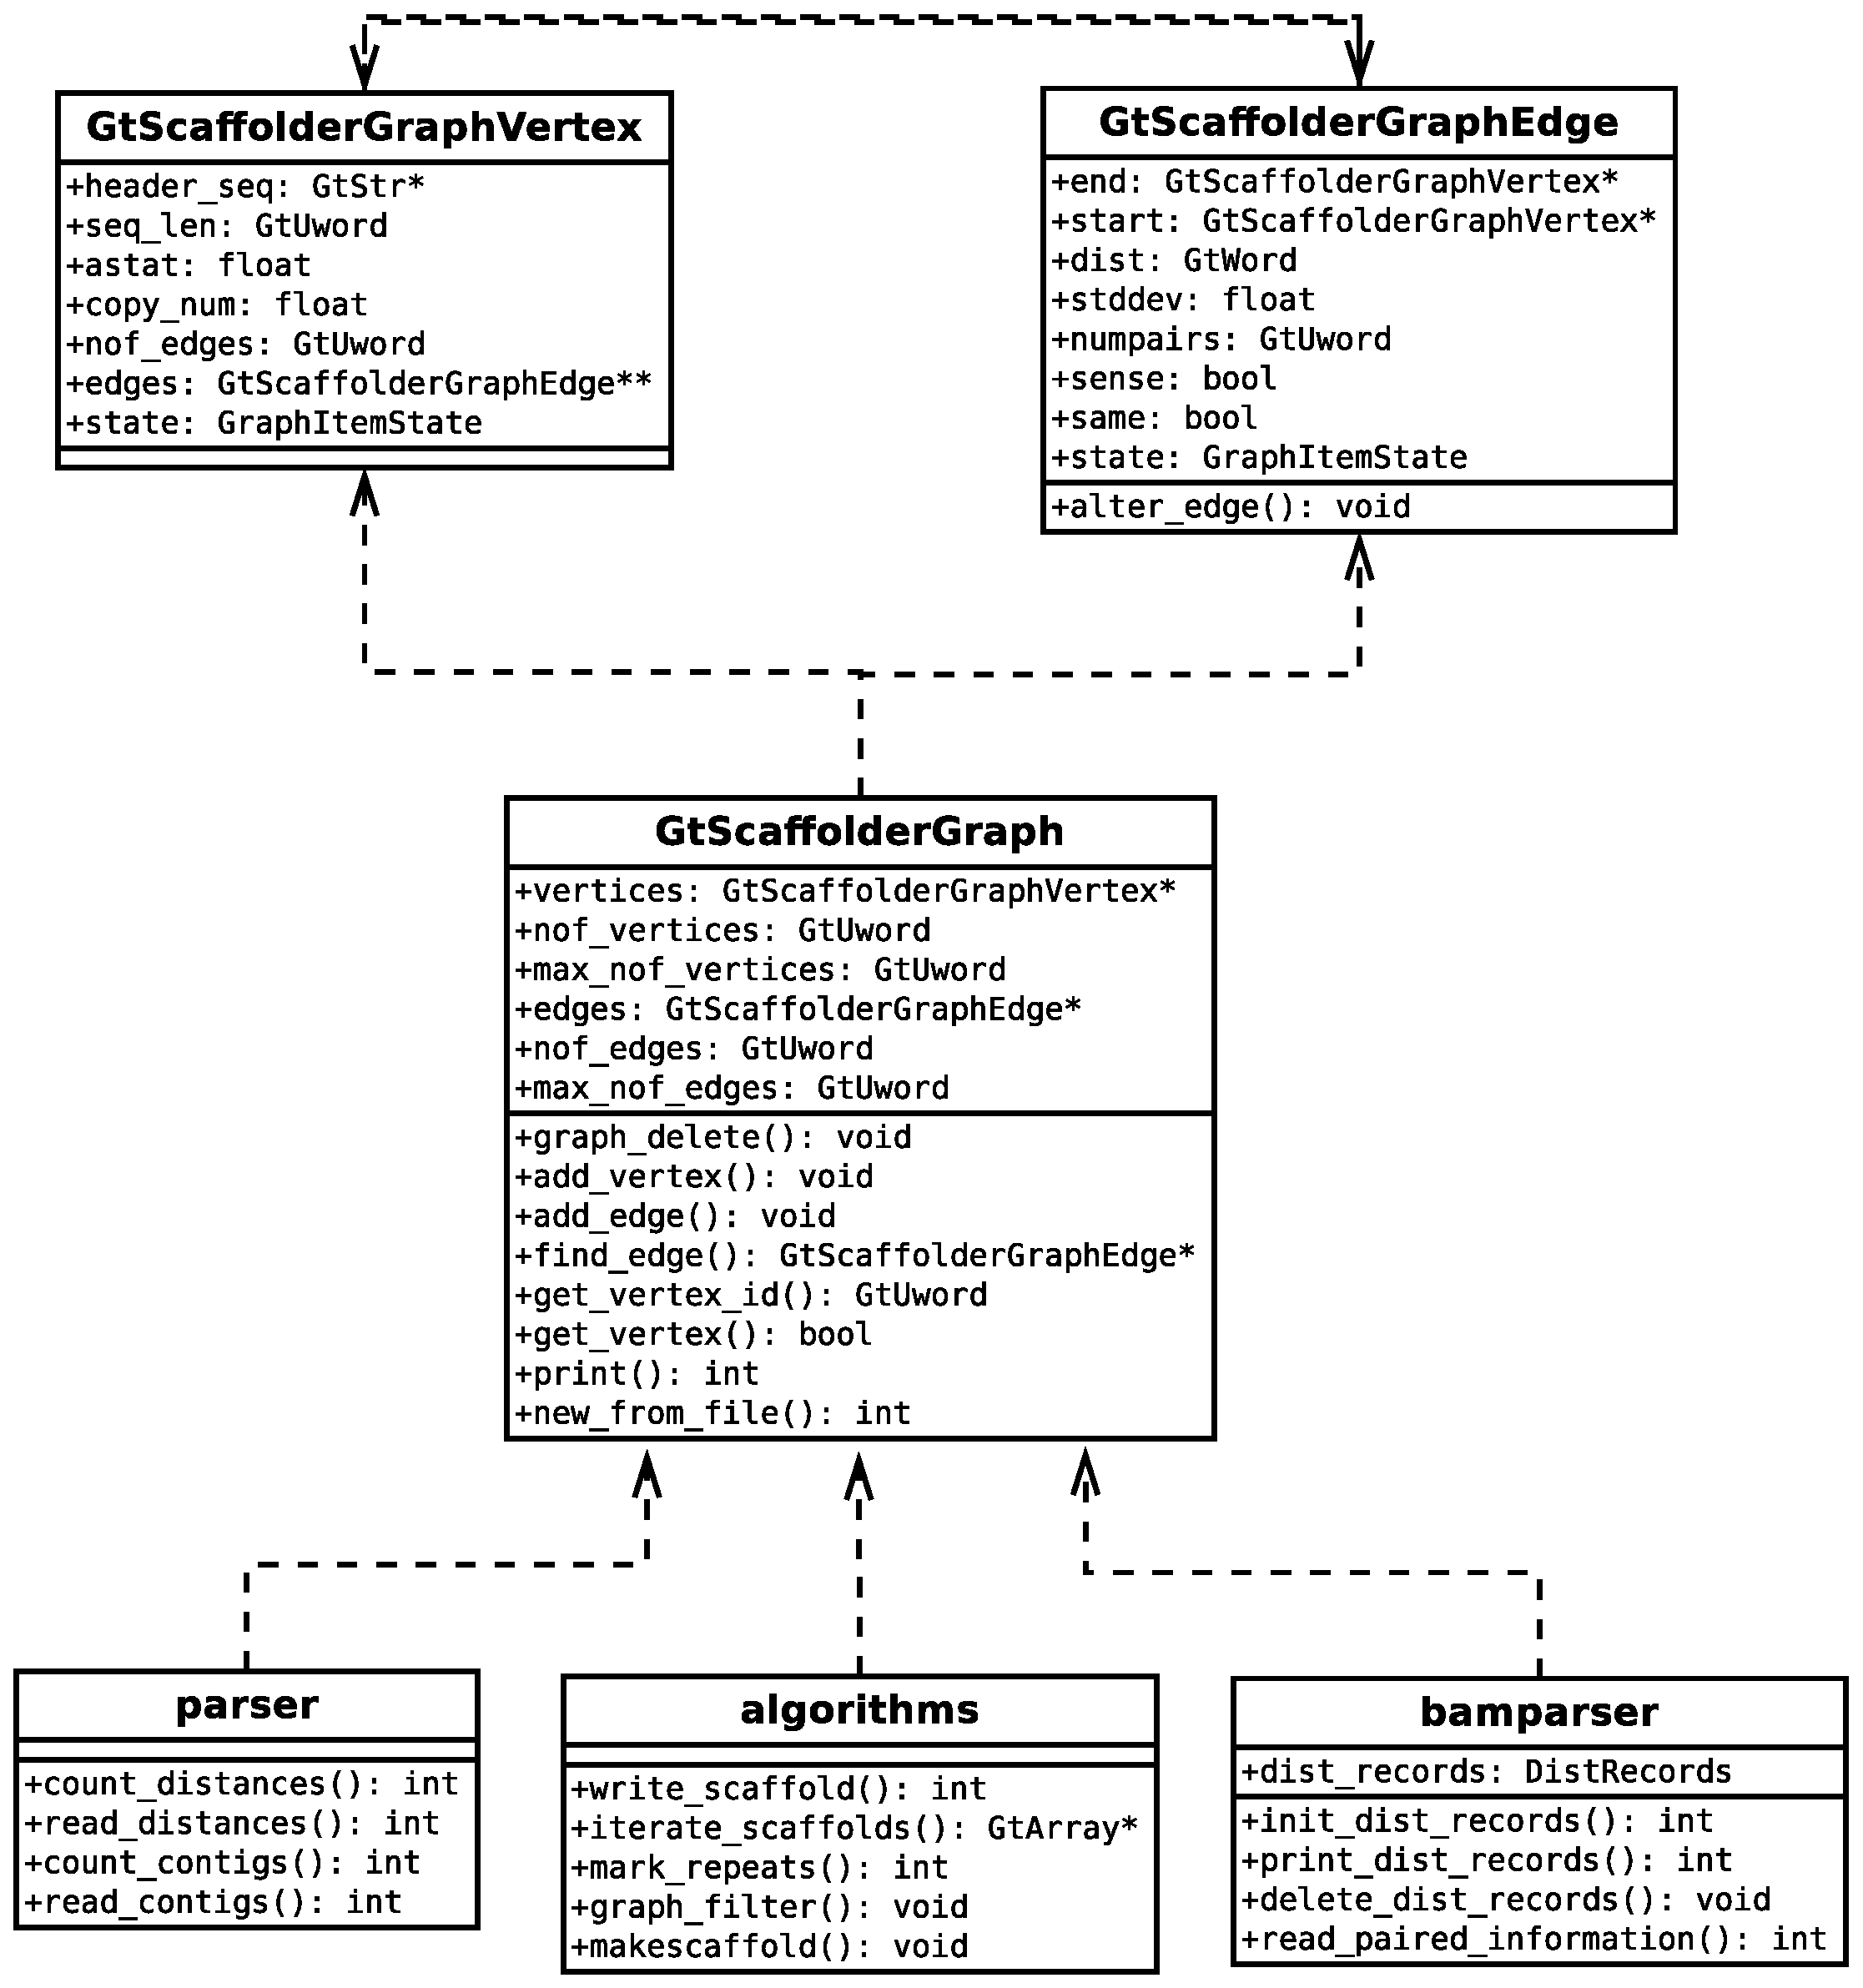
\includegraphics[width=1\linewidth]{uml.eps}
  \caption{Klassendiagramm für gt Scaffolder.}
\label{abb: UML}
\end{figure}

\subsection{gt Scaffolder als Tool in den GenomeTools}
Die Software gt Scaffolder wurde als eigenständiges Tool in die GenomeTools
eingebunden. In Abbildung \ref{abb: help} ist die Ausgabe der Hilfe des Tools
gt Scaffolder dargestellt, in der alle einstellbaren Parameter mit ihren
standardmäßigen Belegungen aufgelistet sind.

\begin{figure}
\begin{verbatim}
$ gt scaffolder -help
Usage: gt scaffolder [option ...] [file]
Constructs scaffolds of the contigs.

-min_contig_len    minimal contig length for used contigs
                   default: 200
-rep_cp_cutoff     minimal copy number for not repetitiv contigs
                   default: 0.30
-rep_astat_cutoff  minimal A-statistics for not repetitiv contigs
                   default: 20.00
-p_cutoff          probability cutoff for polymorphic vertices
                   default: 0.01
-cp_cutoff         copy num cutoff for polymorphic vertices
                   default: 1.50
-overlap_cutoff    overlap cutoff for inconsistent edges
                   default: 400
-contigs           contigs in FASTA format
                   default: undefined
-dist              distanceinformation in ABySS .de format
                   default: undefined
-astat             A-statistics file in SGAs .astat format
                   default: undefined
-spm               basename of spm-representation of used string-graph
                   default: undefined
-bam_min_qual      minimal quality in bam file
                   default: 10
-bam_min_nof_pairs minimal number of pairs
                   default: 10
-bam_min_dist      minimal distance of contigs
                   default: -99
-bam_max_dist      maximal distance of contigs
                   default: infinite
-bam_min_align     minimal alignment length
                   default: 100
-bam               bam file containing alignments of paired reads to the contigs
                   default: undefined
-help              display help and exit
-version           display version information and exit

Report bugs to <gt-users@genometools.org>.
\end{verbatim}
\caption{\label{abb: help}Hilfeausgabe des Tools gt Scaffolder.}
\end{figure}

Beim Aufruf von gt Scaffolder stellen die Optionen -contig und entweder
-dist oder -bam Pflichtangaben dar. Wenn die Übergabe einer Distanzdatei
im ABySS-Distanz-Format (*.de) mit der Option -dist erfolgt, dann wird
diese Datei eingelesen und die enthaltenen Distanzinformationen verwendet.
Gibt man dagegen mit der Option -bam eine BAM-Datei mit Alignments der Reads
zu den Contigs an, so werden aus der BAM-Datei die Distanzinformationen
berechnet und im ABySS-Distanz-Format (*.de) gespeichert. Diese neu erzeugte
Datei wird anschließend eingelesen und die enthaltenen Informationen genutzt.
Die Verwendung einer BAM-Datei und des String-Graph Assemblers Readjoiner
ermöglicht die Abhängigkeit zu einem Mapping-Programm (z.\,B. BWA) und der
Software DistEst von ABySS potentiell zu durchbrechen. So kann Readjoiner die
Daten, auf denen die Alignments der Reads zu den Contigs basieren, direkt
ausgeben. Auf Grund von Zeitmangel existiert jedoch noch kein Modul zur
Konvertierung dieser Daten in eine entsprechende BAM-Datei.

Mit der Option -astat kann zusätzlich eine Datei mit Informationen
über die A-Statistik und die berechneten Kopiezahlen der Contigs
übergeben werden. Diese Option wird für die Kompatibilität mit der
Eingabe von SGA Scaffold benötigt. Wenn diese Option fehlt, besteht die
Annahme, dass diese Informationen innerhalb des Headers der
Contigs vorliegen. Dabei diente das Ausgabeformat für die Contigs von
Readjoiner als Vorlage, das bei Verwendung der Optionen -astat und
-copy$\_$num die A-Statistik und Kopiezahl der Contigs enthält.

Die Standardausgabe stellt eine Datei im SCAF-Format dar. Die
Rekonstruktion der Sequenzen ist in dem Tool noch nicht möglich, da
die Erweiterung der String-Graph-API zur Sequenzkonstruktion mittels
Traversierung des String-Graphen noch nicht in die GenomeTools
übernommen wurde.

\subsection{Strategien in SGA Scaffold mit unklarer Bedeutung}
\label{sec: wunderlich}
SGA benutzt eine relativ konservative Strategie, um vermeintlich
fehlerhafte Knoten und Kanten aus dem Scaffold-Graph zu
entfernen. D.\,h.\ korrekte Knoten und Kanten werden lieber als
fehlerhaft eingestuft und entfernt, als dass fehlerhafte Knoten oder
Kanten nicht erkannt werden und in dem Endergebnis enthalten sein
könnten. Einige nicht sofort ersichtliche Strategien von SGA wurden
zuerst in gt Scaffolder übernommen, um eine Vergleichbarkeit der
Ergebnisse der beiden Programme zu erhalten. Die Güte der Strategien
wurde teilweise evaluiert (siehe Abschnitt~\ref{sec: Ergebnisse}).

Es folgt eine ungeordnete Auflistung solcher Strategien, teilweise um
mögliche Erklärungen ergänzt.
\begin{itemize}
\item Bei der Entfernung inkonsistenter Kanten eines Knoten $k_0$
  werden alle Kanten von den Nachbarknoten, die in der gleichen
  Richtung (\textit{sense} oder \textit{antisense}) verlaufen wie die
  Kante vom Nachbarknoten zu $k_0$, ebenfalls entfernt. \\
  Mögliche Erklärung: Potentiell enthalten auch diese Kanten
  Inkonsistenzen und sollten deshalb nicht weiter betrachtet werden.
\item Bei der Konstruktion des Graphen werden zwischen zwei Knoten
  jeweils nur zwei Kante eingefügt, eine Hin- und eine Rückkante.
  Wenn es mehr als ein mögliches Kantenpaar gibt, wird das Kantenpaar mit der
  größten Standardabweichung gewählt. \\
  Mögliche Erklärung: keine.
\item Bei der Klassifikation der Knoten als repetitiv oder eindeutig
  wird zusätzlich zu der A-Statistik auch die berechnete Anzahl an
  Kopien für jeden repräsentierten Contig betrachtet. Ein Knoten wird
  dabei als repetitiv markiert und später entfernt, wenn die
  berechnete Anzahl an Kopien für den repräsentierten Contig zu gering
  ist. \\
  Mögliche Erklärung: Die Contigs mit einer zu geringen
  Kopiezahl sind potentiell fehlerhaft und sollten nicht betrachtet
  werden. Die Markierung als repetitiv ist dabei semantisch falsch und
  dient nur der späteren Entfernung des zugehörigen Knoten.
\end{itemize}

\section{Ergebnisse}
\label{sec: Ergebnisse}
\subsection{Gegenüberstellung der Pipelines}

\begin{figure}
  \centering
  \begin{minipage}{.45\textwidth}
      \begin{tikzpicture}[node distance=.8cm]
        \tikzstyle{prog}=[draw, rectangle, rounded corners];
        \node[prog] (prep) {preprocess};
        \node[prog, below of=prep] (index) {index};
        \node[prog, below of=index] (correct) {correct};
        \node[prog, below of=correct] (index2) {index};
        \node[prog, below of=index2] (filter) {filter};
        \node[prog, below of=filter] (overlap) {overlap};
        \node[prog, below of=overlap] (assemble) {assemble};
        \node[prog, right of=prep, xshift=2cm, fill=red!40] (bindex) {index};
        \node[prog, below of=bindex, fill=red!40] (aln) {align};
        \node[prog, below of=aln, fill=red!40] (sampe) {sampe};
        \node[prog, below of=sampe, rectangle split, rectangle split parts=3, yshift=-.45cm, rectangle split part fill={blue!40, green!40, blue!40}] (bam2de) {\nodepart{one}fixmate\nodepart{two}samtools\nodepart{three}DistanceEst};
        \node[prog, below of=bam2de, yshift=-.45cm, fill=yellow!40] (pysam) {astat};
        \node[prog, below of=pysam] (scaff) {scaffold};
        \node[prog, below of=scaff] (scaf2fasta) {scaf2fasta};

        \path[->]
        (prep) edge (index)
        (index) edge (correct)
        (correct) edge (index2)
        (index2) edge (filter)
        (filter) edge (overlap)
        (overlap) edge (assemble)
        (assemble.east) edge[in=180, out=0] (bindex.west)
        (bindex) edge (aln)
        (aln) edge (sampe)
        (sampe) edge (bam2de)
        (bam2de) edge (pysam)
        (pysam) edge (scaff)
        (scaff) edge (scaf2fasta);
      \end{tikzpicture}
    \end{minipage}
    \begin{minipage}{2cm}
      \begin{tikzpicture}[node distance=.8cm]
        \tikzstyle{prog}=[draw, rectangle, rounded corners];
        \node[prog] (prefilter) {prefilter};
        \node[prog, below of=prefilter] (overlap) {overlap};
        \node[prog, below of=overlap] (assembly) {assembly};
        \node[prog, right of=prefilter, xshift=1.5cm] (scaffold) {scaffold};

        \path[->]
        (prefilter) edge (overlap)
        (overlap) edge (assembly)
        (assembly.east) edge[in=180, out=0] (scaffold.west);
      \end{tikzpicture}
    \end{minipage}
    \caption{\label{abb: Pipeline}Vergleich der Assemblierungs- und
      Scaffolding-Pipelines von SGA (links) und gt Scaffolder
      (rechts). Externe Abhängigkeiten zu unterschiedlichen Programmen
      oder Bibliotheken sind jeweils in unterschiedlichen Farben
      hervorgehoben. Innerhalb jeder Pipeline sind die zur Assemblierung
      notwendigen Schritte links, die für das Scaffolding ausgeführten Schritte
      rechts angeordnet.}
\end{figure}

Auf der jeweils linken Seite sind die notwendigen Schritte zur
Assemblierung dargestellt und auf der rechten Seite die Schritte für
das Scaffolding. In der linken Abbildung ist die SGA-Pipeline zu sehen
und in der rechten Abbildung die Pipeline aus dem Assemblierer
Readjoiner und gt Scaffolder. Die rechte Pipeline funktioniert noch
nicht komplett, da einige in Readjoiner intern vorhandene
Informationen in den richtigen Formaten mit ausgegeben werden müssen.

In der Abbildung ist zu erkennen, dass SGA wesentlich mehr Schritte
sowohl bei der Assemblierung als auch beim Scaffolding
durchläuft. Zusätzlich enthält die Pipeline Abhängigkeiten von
nicht-Standardsoftware, in der Abbildung farbig markiert. Die
unterschiedlichen Farben kennzeichnen unterschiedliche Programme und
Bibliotheken, zu denen Abhängigkeiten bestehen.

Ein Vergleich der \textit{de novo}-Assemblierungs-Pipelines von SGA und gt
Scaffolder (vgl. Abbildung~\ref{abb: Pipeline}) zeigt wesentliche Unterschiede
in der Anzahl der benötigten Schritte sowie externen Abhängigkeiten auf.
SGA durchläuft sowohl bei der Assemblierung als auch beim Scaffolding wesentlich
mehr Schritte. Gleichzeitig besitzt die SGA-Pipeline externe Abhängigkeiten,
was ihre Komplexität noch erhöht: Neben der Software ABySS, BWA, SAMtools und
ihren Kompilierungsabhängigkeiten müssen externe Bibliotheken wie Pysam
vorliegen, da manche Schritte der SGA-Pipeline von Perl- und Python-Skripten
verwaltet werden.
gt Scaffolder besitzt für die Assemblierung eine GenomeTools-interne
Abhängigkeit zur gt Readjoiner. Zum Zeitpunkt dieser Ausarbeitung ist die
Schnittstelle zu Readjoiner noch nicht vollständig implementiert
(vgl. Abschnitt~\ref{sec: Ausblick}). Darüber hinaus ist gt Scaffolder zur
SGA-Pipeline kompatibel und kann dieselben Eingabedaten verarbeiten wie
SGA-Scaffold.

\subsection{Scaffold-Berechnung durch gt Scaffolder und SGA im Vergleich}
Zur Überprüfung und Evaluation wurden Scaffolds für verschiedene Testdaten durch
gt Scaffolder berechnet. Zur besseren Einordnung der Ergebnisse wurde eine
Scaffold-Berechnung ebenfalls mit SGA durchgeführt. Die Berechnungen wurden auf
einem Computer mit 3.10GHz Intel Core-i7 Prozessor, 8GB Arbeitsspeicher unter
einem 64bit Linux Betriebssystem ausgeführt. Dabei wurde lediglich ein Kern
verwendet. Das Laufzeitverhaltens und der Speicherbedarf wurden durch das in den
GenomeTools enthaltene Skript rdj-spacepeak.sh auf auf 2 identischen Computern
gemessen, um eine eventuelle Verfälschung durch das
Caching der Eingabedateien zu vermeiden. Die von beiden Programmen ausgegebenen
Metriken wurden durch gt seqstat nochmals überprüft. Bei der
Rekonstruktion der Sequenzen aus den ermittelten Scaffolds handelt es sich um
einen separaten Schritt, der gesondert ausgewertet wurde. Hier wurden die
Metriken durch QUAST~\cite{Gurevich:2013je} ermittelt.

\subsubsection*{Generierung und Assemblierung der Testdaten}
Mithilfe der Software ART~\cite{Huang:2012kq} wurde eine
Illumina-\textit{Paired-End}-Sequenzierung für vier verschiedene Referenzgenome
(vgl. Tabelle~\ref{tab: Referenzgenome}) simuliert. Dabei wurde die Read-Länge
auf 150 bp, die Fragmentlänge auf 400 bp $\pm$ 10 bp und die Coverage auf
20X festgelegt sowie der Seed 123 gewählt. Die Längen der Referenzgenome
variieren im Bereich von ca. 10 bis 140 Mbp, um die Entwicklung der Laufzeit
und des Speicherbedarfs mit steigender Länge beobachten zu können.
Getestete, kürzere Zielsequenzen konnten teilweise bereits während der
Assemblierung vollständig rekonstruiert werden.

Anschließend wurden die simulierten \textit{Paired-End}-Reads aller vier
Datensätze jeweils durch die SGA-Pipeline (vgl. Abbildung~\ref{abb: Pipeline})
assembliert, bevor die komparative Scaffold-Berechnung durchgeführt wurde.

\begin{table}
  \centering
  \begin{tabular}{lcl}
    Genom & Größe (Mbp) & Ensemble Build \\
    \hline
    \textit{S. cerevisiae} &~~12 & R64-1-1 \\
    \textit{H. sapiens}, Chr. 21 &~~48 & GRCh37 \\
    \textit{C. elegans} & 100 & WBcel235 \\
    \textit{D. melanogaster} & 140 & BDGP5
  \end{tabular}
  \caption{\label{tab: Referenzgenome}Verwendete Referenzgenome mit ihrer
  Größe. Alle Sequenzen stammen aus dem Ensemble-Projekt (www.ensembl.org),
  die jeweilige Build-Nummer ist angegeben.}
\end{table}

\subsubsection*{Ergebnisse der Scaffold-Berechnung}

Für alle 4 Testdatensätze konnte gt Scaffolder eine erfolgreiche
Scaffold-Berechnung durchführen. Ein Vergleich mit SGA (vgl.
Tabelle~\ref{tab: Scaffolding}) zeigt das Güte der Ergebnisse für die
betrachteten Metriken exakt übereinstimmen. Die Abdeckung der
jeweiligen Zielsequenz durch die Gesamtlänge der ermittelten Scaffolds
schwankt zwischen 71 und 94\%. Eine Korrelation mit der Genomlänge
oder Anzahl der in den Scaffolding-Schritt eingehenden Contigs ist
hierbei nicht vorhanden.

Insgesamt war gt Scaffolder mindestens genauso oder etwas performanter als
SGA (vgl. Abbildung~\ref{abb: Zeit}). Der Laufzeitbedarf betrug für alle
Berechnung nur einige Millisekunden, der maximale Speicherbedarf etwa 30 MB. gt
Scaffolder war dabei etwa gleich schnell oder um den Faktor $0.9\times$
schneller als SGA. Der Speicherbedarf während der Berechnung durch gt
Scaffolder war um den Faktor $0.90\times$ bis $0.43\times$ geringer.

\begin{table}
  \adjustbox{max height=\dimexpr\textheight-5.5cm\relax, max width=\textwidth}{
    \begin{tabular}{llccccc}
      \toprule
      Datensatz & Programm & Abdeckung (Mbp / \%) & \#Scaffolds & N50 (kb) & CPU (s) & RAM (MB) \\
      \midrule
      \textit{S. cerevisiae}
      & SGA Scaffold  & ~~11.08 / 92  &     ~~600   &  32.3     & 0.01      &  28.9 \\
      1694 contigs
      & gt Scaffolder & $1\times$     &  $1\times$  & $1\times$ & $1\times$ &  $0.43\times$ \\
      \midrule
      \textit{H. sapiens}, Chr. 21
      & SGA Scaffold  & ~~34.25 / 71  &      1368   &  54.2     & 0.04  &  27.8  \\
      4817 contigs
      & gt Scaffolder & $1\times$     &  $1\times$  & $1\times$ & $1\times$ & $0.6\times$       \\
      \midrule
      \textit{C. elegans}
      & SGA Scaffold  & ~~94.07 / 94  &      5659   &  36.9     & 0.11  &  34.9 \\
      11113 contigs
      & gt Scaffolder & $1\times$     &  $1\times$  & $1\times$ & $0.9\times$ & $0.90\times$      \\
      \midrule
      \textit{D. melanogaster}
      & SGA Scaffold  & 113.48 / 81   &      2281   &  126.3    & 0.11    & 29.2     \\
      3970 contigs
      & gt Scaffolder & $1\times$     &  $1\times$  & $1\times$ & $0.9\times$ & $0.62\times$     \\
      \bottomrule
  \end{tabular}}
  \caption{\label{tab: Scaffolding}Ergebnisse der Scaffold-Berechnung.
  Datensatz bezeichnet die Testdatensätze mit zugehöriger Anzahl der
  assemblierten Contigs, um die Größe des jeweiligen Scaffold-Graphen zu
  skizzieren. Für jeden Datensatz wurden die zunächst die durch SGA erzielten
  Ergebnisse aufgetragen in der ersten Zeile als absolute Werte aufgetragen,
  denen die Ergebnisse von gt Scaffolder in der zweiten Zeile als relative
  Faktoren folgen. Abdeckung bezeichnet Gesamtlänge aller Scaffolds und die
  prozentuale Abdeckung der Zielsequenz, \#Scaffolds
  deren Anzahl und N50 die Länge, sodass alle  Scaffolds mit gleicher oder
  größerer Länge mindestens die Hälfte der Abdeckung ausmachen. CPU bezeichnet
  die Gesamtlaufzeit und RAM den maximalen Speicherbedarf während der
  Berechnung.}
\end{table}

\begin{figure}[t]
  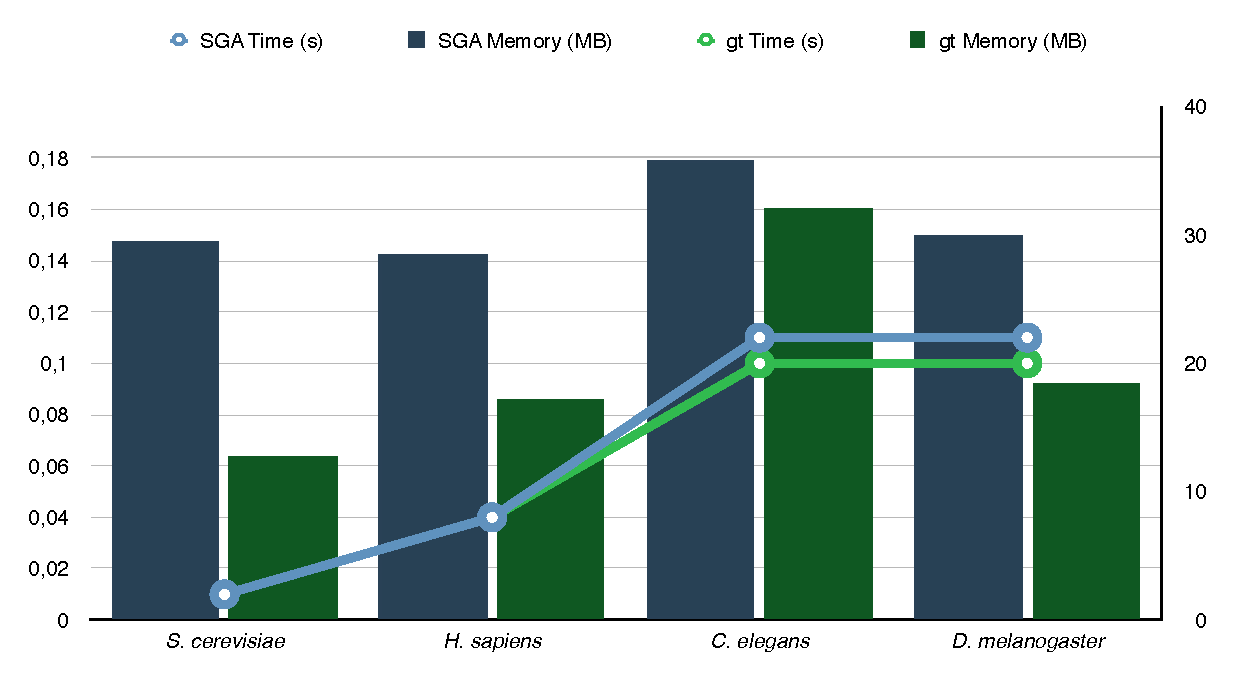
\includegraphics[width=\textwidth,height=0.8\textheight,keepaspectratio]{presentation/figures/sga_vs_gt.pdf}
  \caption{\label{abb: Zeit}Graphische Darstellung der Laufzeit (Graphen) und
  des Speicherplatzbedarfs (Balkendiagramme) von gt Scaffolder (grün) und SGA
  Scaffold (rot) für die nach Größe geordneten Testdatensätze. }
\end{figure}


\subsubsection*{Ergebnisse der Sequenz-Rekonstruktion}
Während gt Scaffolder die Scaffold-Berechnung und Rekonstruktion der Zielsequenz
in einem Schritt berechnen kann, handelt es sich bei SGA um 2 getrennte
Schritte: SGA Scaffold und SGA scaffold2fasta. Für alle 4 Testdatensätze konnte
gt Scaffolder eine Sequenz-Rekonstruktion durchführen. Im Gegensatz zur
Scaffold-Berechnung existieren hier wesentlich Unterschiede zu den mit SGA
rekonstruierten Sequenzen (vgl. Tabelle~\ref{tab: Rekonstruktion}), welche das
jeweilige Referenzgenom deutlich besser abdecken und gleichzeitig weniger
missassemblierte Positionen besitzen.

\begin{table}
  \adjustbox{max height=\dimexpr\textheight-5.5cm\relax, max width=\textwidth}{
    \begin{tabular}{llccccc}
      \toprule
      Datensatz & Programm & Gesamtlänge (Mbp) & Abdeckung (\%) & N50 (kb)
      & \#Miss & Unaligniert (bp) \\
      \midrule
      \textit{S. cerevisiae}
      & SGA scaffold2fasta  & 10.91  &    88.9     &  7.9        &
      2 & 0\\
      & gt Scaffolder & $1.1\times$  & $0.4\times$ & $1.2\times$ &
      $1587.5\times$ & \\
      \midrule
      \textit{H. sapiens}, Chr. 21
      & SGA scaffold2fasta  & 34.32  &      73.1   &  54.3       &
      1 & 535\\
      & gt Scaffolder & $0.3\times$  & $0.3\times$ & $0.2\times$ &
      $2114\times$ & $1\times$\\
      \midrule
      \textit{C. elegans}
      & SGA scaffold2fasta  & 94.78  &      90.3   &  37.4       &
      13 & 3301 \\
      & gt Scaffolder & $0.5\times$  & $0.5\times$ & $0.4\times$ &
      $167.9\times$ & $18.2\times$\\
      \midrule
      \textit{D. melanogaster}
      & SGA scaffold2fasta  & 113.50 &      94.2   &  126.4      &
      1  & 0 \\
      & gt Scaffolder & $0.6\times$  & $0.6\times$ & $0.6\times$ &
      $471\times$ & $21871\times$\\
      \bottomrule
  \end{tabular}}
  \caption{\label{tab: Rekonstruktion}Ergebnisse der Sequenz-Rekonstruktion.
  Datensatz bezeichnet die Testdatensätze mit zugehöriger Anzahl der
  assemblierten Contigs, um die Größe des jeweiligen Scaffold-Graphen zu
  skizzieren. Für jeden Datensatz wurden die zunächst die durch SGA erzielten
  Ergebnisse aufgetragen in der ersten Zeile als absolute Werte aufgetragen,
  denen die Ergebnisse von gt Scaffolder in der zweiten Zeile als relative
  Faktoren folgen. Abdeckung bezeichnet Gesamtlänge aller Scaffolds, Abdeckung
  die prozentuale Abdeckung der Zielsequenz und N50 die Länge, sodass alle
  Scaffolds mit gleicher oder größerer Länge mindestens die Hälfte der
  Gesamtlänge ausmachen. \#Miss bezeichnet die Anzahl der
  Missassemblierungen nach Plantagora \cite{Gurevich:2013je}, Unaligniert die
  Gesamtlänge nicht alignierter Regionen der Assemblierungen.}
\end{table}


\section{Diskussion}
\label{sec: Diskussion}

Wie in Abschnitt \ref{sec: Ergebnisse} dargestellt, liefert gt
Scaffolder in den Testfällen die gleichen Ergebnisse wie SGA
Scaffold. Dabei benötigt gt Scaffolder die gleiche Laufzeit und
weniger Speicherplatz.

Aus den Ergebnissen im Vergleich der Ausgabe im SCAF-Format ist zu
erkennen, dass die Laufzeit und der Speicherplatzbedarf nicht mit der
Größe der Referenzgenome zusammenhängt. Allerdings hängen diese
Aspekte auch nicht direkt von der Größe des Scaffold-Graphen ab. In
Tabelle \ref{tab: Scaffolding} sind zu den Datensätzen die Anzahl an
Knoten in dem Scaffold-Graph dargestellt. So ist die Anzahl an Knoten
für den \textit{D. melanogaster} Datensatz mit $3970$ geringer als für
den \textit{H. sapiens} Chr. 21 Datensatz mit $4817$ Knoten. Trotzdem
wird zur Berechnung der Scaffolds für den \textit{D. melanogaster}
Datensatz sowohl von SGA Scaffold als auch von gt Scaffolder mehr
Laufzeit und mehr Speicherplatz benötigt, wie aus Tabelle \ref{tab:
  Vergleich} und Abbildung \ref{abb: Zeit} ersichtlich wird.

Das Modul zur Rekonstruktion der Sequenzen ist scheinbar noch
fehlerhaft und liefert keine vergleichbar gute Ergebnisse wie das
äquivalente Modul von SGA. Dies kann dadurch kommen, das SGA den
String-Graph nach dem Einlesen noch modifiziert und ebenfalls Lücken
mit negativer Distanz anhand des String-Graphen schließt. Ebenfalls
verwendet SGA eine andere Strategie zur Berechnung von Alignments. Bei
dieser Berechnung verwendet das Modul von gt Scaffolder ein
Distanz-Modell. SGA hingegen verwendet ein
Ähnlichkeits-Scoring-Modell, welches übereinstimmende Buchstaben
stärker positiv bewertet. Zusätzlich kann das Modul von gt Scaffolder
die nicht im Scaffolding enthaltenen Contigs noch nicht mit
ausgeben. SGA gibt kann diese Contigs mit ausgeben und erreicht
dadurch gegebenenfalls eine höhere Abdeckung des Referenzgenoms.

SGA-Scaffold hat viele Parameter und Optionen für das Scaffolding. So
kann die Strategie für die Auswahl der relevanten Knoten und Kanten
ausgewählt werden. gt Scaffolder implementiert hingegen nur eine
dieser möglichen Optionen. Die meisten Parameter, die bei SGA-Scaffold
gewählt werden können, sind auch bei gt Scaffolder einstellbar. Somit
ist SGA-Scaffold flexibler in der Selektion relevanter Kanten und
Knoten als gt Scaffolder.

Die Wahl der Programmiersprache C für gt Scaffolder war gut im
Vergleich zu einer Implementierung der Scaffolding-Software in einer
Skriptsprache wie z.\,B. Python, Ruby oder Perl. Bei einer
Implementation in einer Skriptsprache wäre das Einlesen der
verschiedenen Format wesentlich einfacher gewesen und die
Implementation schneller beendet, da Stringmanipulation in diesen
Sprachen nicht so aufwändig ist. Allerdings hätte die in den
GenomeTools vorhandene Infrastruktur nicht so einfach genutzt werden
können. So hätte vor allem die Implementation des Moduls zur
Rekonstruktion der Sequenzen länger gedauert. Es hätten
Datenstrukturen wie der String-Graph nutzbar gemacht oder neu
implementiert werden müssen. Ebenfalls hätten vorhandene
Implementationen von Algorithmen wie z.\,B. die Implementation des
Smith-Waterman-Algorithmus zur Berechnung lokaler Alignments nicht
einfach genutzt werden können. Der geringere Verbrauch an
Speicherplatz wäre in einer Skriptsprache wahrscheinlich nicht möglich
gewesen. Durch die Infrastruktur der GenomeTools waren Datenstrukturen
wie z.\,B. Arrays, Queues oder Hashes schon vorhanden. Dadurch war die
Nutzung solcher Datenstrukturen vergleichbar komfortabel mit einer
Skriptsprache.

\section{Ausblick}
\label{sec: Ausblick}

Die Scaffolding-Software gt Scaffolder kann um viele Optionen
erweitert werden. So können weitere Strategien zur Selektion
relevanter Knoten und Kanten implementiert werden, um für den
jeweiligen Datensatz eine gute Lösung produzieren zu
können. Z.\,B. können weitere Zyklendetektionsalgorithmen, wie in
SGA-Scaffold, implementiert werden. Ebenso ist in SGA-Scaffold die
Möglichkeit vorhanden transitive Kanten zu entfernen.

Zusätzlich sollten die konservativen Strategien zur Klassifikation in
repetitive bzw. eindeutige Knoten untersucht werden. Durch besser
gewählte Schwellenwerte könnten bessere Ergebnisse erzielt werden. Die
in Abschnitt \ref{sec: wunderlich} dokumentierten Strategien sollten
ebenfalls überprüft werden.

gt Scaffolder bietet zudem einen Ausgangspunkt für eine Laufzeit- und
Speicherplatzoptimierung. Die Ergebnisse bezüglich dieser Aspekte sind
schon vielversprechend und könnten noch weiter optimiert werden. Für
eine Laufzeitoptimierung ist eine Parallelisierung einiger Schritte
möglich. So ist die Berechnung der einzelnen Scaffolds unabhängig
voneinander, da diese für die einzelnen Zusammenhangskomponenten
berechnet werden. Nach der Ermittlung der Zusammenhangskomponenten
könnten die Zyklendetektion und später das eigentliche Scaffolding für
jede Zusammenhangskomponente in einem eigenen Thread durchgeführt
werden. Durch die Verwendung effizienterer Datenstrukturen können
ebenfalls Laufzeit und Speicherplatzbedarf eingespart werden. Der
Fokus der hier beschriebenen Implementation lag nicht auf Laufzeit-
und Speicherplatzeffizienz.

Wie in Abschnitt \ref{sec: Ergebnisse} aufgezeigt ist die
Implementation des Moduls zur Rekonstruktion der Sequenzen
verbesserungsbedürftig. Bei der Rekonstruktion der Sequenzen können
die durch gt Scaffolder erzeugten Scaffolds im SCAF-Format genutzt
werden. Die Strategie um die Sequenzen zu rekonstruieren kann dabei
von SGA adaptiert werden oder eine andere Strategie genutzt werden.

Die Ausgaben des in den GenomeTools enthaltenen Assemblers Readjoiner
müssen teilweise noch verändert werden um eine Nutzung mit gt
Scaffolder in einer Pipeline zu ermöglichen. So müssen die
Mapping-Informationen über die Reads zu den Contigs in das BAM-Format
übertragen werden. Dabei ist das BAM-Format ein Standardformat und es
könnte sowohl Readjoiner um eine Ausgabe im BAM-Format erweitert oder
ein Skript zur Transformation der Information in das benötigte Format
genutzt werden.

Die Standardwerte für die einzelnen Parameter müssen bei einer
Benutzung mit Readjoiner auf dessen Ergebnisse eingestellt werden. Die
momentan verwendeten Standardwerte sind von SGA übernommen und
dementsprechend auf die Ergebnisse der SGA-Pipeline optimiert. Da
Readjoiner z.\,B. andere Ergebnisse bei der Berechnung der A-Statistik
erreicht, müsste der Schwellenwert zur Klassifikation als nicht
repetitive Sequenz angepasst werden.

\section*{Anhang}
\subsection*{Pseudocode}

\begin{algorithm}
  \ForEach{Knoten $k_0$ im Graph $G$}{
    \ForEach{Kantenrichtung $dir$ in [ANTISENSE, SENSE]}{
      \ForEach{Kantenpaar $(e_0,e_1)$ in Richtung $dir$}{
        $k_1$ = $e_0.end$\;
        $k_2$ = $e_1.end$\;
        \If{AmbiguousOrdering($e_0,e_1,p\_cutoff$) \textbf{and}
           $k_1.copy\_num + k_2.copy\_num < cn\_cutoff$}
          {
            \If{$k_1.copy\_num < k_2.copy\_num$}{
              markiere $k_1$ und alle ein- und ausgehenden Kanten
              von $k_1$ als polymorph, wenn $k_1$ noch nicht markiert
              ist\;
            }
            \Else {
              markiere $k_2$ und alle ein- und ausgehenden Kanten
              von $k_2$ als polymorph, wenn $k_2$ noch nicht markiert
              ist\;
            }
          }
        }
      \tcp{polymorphe Knoten müssen nicht mehr auf
        inkonsistente Kanten überprüft werden}
       \If{Knoten $k_0$ ist polymorph}
         {break\;}
       \ForEach{Kantenpaar $(e_0,e_1)$ in Richtung $dir$}{
         \If{$e_0$ ist nicht markiert und $e_1$ ist nicht markiert}
            {
              Berechne Überlappung von $e_0.end$ und $e_1.end$ und speichere
              längsten Überlappung.\;
            }
       }
       \If{längste Überlappung $>$ 400} {
          Markiere alle ausgehenden Sense- bzw. Antisensekanten
          von $k_0$ und die eingehenden Kanten mit der Richtung der
          jeweiligen Zwillingskante als inkonsistent\;
      }
    }
  }
  \caption{\label{alg: Selektion}Filterfunktion zur Markierung von
    polymorphen Knoten und inkonsistenten Kanten. Die Funktion
    \textit{AmbigousOrdering} ist in Algorithmus \ref{alg: Order}
    dargestellt.}
\end{algorithm}

\begin{algorithm}
  \KwData{Kante $e_0$ und Kante $e_1$, die auf eindeutige Ordnung geprüft werden
    sollen. Wahrscheinlichkeitsschwellenwert $p\_cutoff$}
  \KwResult{Ob die Kanten $e_0$ und $e_1$ nicht eindeutig geordnet werden können}
  $\mu = e_0.dist - e_1.dist$\;
  $\sigma^2 = e_0.std\_dev^2 + e_1.std\_dev^2$\;
  $t = \frac{-\mu}{\sigma\cdot\sqrt{2}}$\;
  $P_{e_0,e_1} = \frac{1}{2} \cdot \left( 1 + \frac{2}{\sqrt{\pi}} \int_{0}^{t} \exp{-x^2}\mathrm dx\right)$\;
  $P_{e_1,e_0} = 1 - P_{e_0,e_1}$\;
  \Return $\max\{P_{e_0,e_1}, P_{e_1,e_0}\} \leq p\_cutoff$
  \caption{\label{alg: Order}Funktion \textsc{AmbiguousOrdering}$(e_0, e_1, p\_cutoff)$}
\end{algorithm}


\begin{algorithm}
  \KwData{Graph}
  \KwResult{Graph ohne Zyklen}
  \While{Zyklus gefunden wurde}{
  Suche alle Zusammenhangskomponenten $CC$\;
  \ForEach{Zusammenhangskomponente $C_0 \in CC$}{
    Suche alle terminalen Knoten $T$\;
    \ForEach{terminalen Knoten $t_0 \in T$}{
      Suche mit einer Tiefensuche von dem Knoten $t_0$ aus in der
      Richtung $t_0.edges[0].sense$ nach Rückkanten\;
      \If{Rückkante gefunden}{
        Markiere die Rückkante und die dadurch verbundenen Knoten
        als zyklisch\;
        }
      }
    }
  }
  \caption{\label{alg: Zyklen}Löse alle Zyklen für jede
    Zusammenhangskomponente auf}
\end{algorithm}

\begin{algorithm}
  \SetAlgoLined
  \KwData{Graph $G$}
  \KwResult{Graph $G$ mit Knoten der Scaffolds markiert}
  Suche alle Zusammenhangskomponenten $CC$\;
  \ForEach{Zusammenhangskomponente $C_0\in CC$}{
    Berechne die Menge der terminalen Knoten $T$ für $C_0$\;
    \ForEach{terminalen Knoten $t_0  \in T$}{
      Berechne die Menge $W$ aller Pfade durch $C_0$ von $t_0$ aus\;
      \ForEach{Pfad $w_0$ aus $W$}{
        \If{Contig-Gesamtlänge > bislang beste Contig-Gesamtlänge}{
          Setze aktuellen Pfad $w_0$ als besten Pfad\;
        }
      }
    }
    Markiere alle Knoten und Kanten entlang des besten Pfades als Scaffold\;
  }
  \caption{\label{alg: Scaffold}Berechnung der Scaffolds. Die
    Berechnung aller Pfade ist in Algorithmus \ref{alg: Pfade} dargestellt.}
\end{algorithm}

\begin{algorithm}
  \SetAlgoLined
  \KwData{terminaler Startknoten $t_0$}
  \KwResult{Alle von diesem Knoten möglichen Pfade}
  Konstruktionsrichtung = $t_0.edges[0].sense$\;
  \ForEach{Kante $e_1$ vom Knoten $t_0$ ausgehend}{
    $k_0$ = $e_1.end$\;
    Speichere Startkante $e_1$ und Distanz $e_1.dist$ in Map an Position
    $k_0$\;
    Schiebe Startkante $e_1$ und Distanz $e_1.dist$ in Queue\;
  }
  \While{BFS über Queue nicht beendet}{
    Poppe Kante $e$ und Distanz $dist$ aus der Queue\;
    $k$ = $e.end$\;
    \ForEach{Kante $e_2$ in Konstruktionsrichtung von $k$ aus} {
      $k_1$ = $e_2.end$\;
      \If{Distanz ($e_2.dist + dist$) zu aktuell betrachtetem Knoten $k_1$ $<$
        bisher ermittelte Distanz zu $k_1$ {\bf OR} Knoten $k_1$
        noch unbetrachtet}{
        Speichere Kante $e_2$ und Distanz $e_2.dist + dist$ in Map an Position $k_1$\;
        Schiebe Kante $e_2$ und Distanz $e_2.dist + dist$ in Queue\;
      }
      neue Konstruktionrichtung = $e_2.twin.sense$\;
    }
    \If{$k$ hat keine Kanten in Konstruktionsrichtung {\bf AND}
    $k$ ist terminal}{
      Schiebe Knoten $k$ in terminalSet $S$\;
    }
  }
  \ForEach{Knoten $k\in S$}{
    Erzeuge Pfad von $t_0$ zu $k$ mithilfe einer Rücktraversierung über die Map\;
  }
  \caption{\label{alg: Pfade}Berechnung aller Pfad zwischen einem
    terminalen Knoten und allen anderen terminalen Knoten einer
    Zusammenhangskomponente}
\end{algorithm}

\bibliography{presentation/literatur}
\bibliographystyle{alpha}

\end{document}
